% chapter 1
\chapter{Introduction}
\label{chap1}


\section{Hardware-based Security}
This chapter provides an introduction to the Hardware-based
Security components, which are essential to build trust 
at the physical level of a system; they protect against
attacks that can't be mitigated by software alone.

\subsection{Hardware Trust}
Hardware trust is a critical aspect of modern computing systems,
ensuring that the hardware components are genuine and have not been
tampered with. 

This trust is established through various mechanisms, including
secure boot processes, hardware root of trust, and the use of
trusted platform modules (TPMs).

\subsection{Root of Trust}
The root of trust is a foundational component in hardware security,
providing a secure anchor for the system's integrity.
It is responsible for verifying the authenticity of hardware and
software components during the boot process.
This component is needed to always behave in the expected way,
because its misbehavior cannot be detected by the system itself.

\subsection{Trust Anchor}
A trust anchor serves as a fundamental element in establishing 
trust within a system. Rather than relying on external validation, 
such as a certificate authority, a trust anchor is typically embedded 
directly into hardware or software, or provisioned securely through 
dedicated channels.

\section{Trusted Platform Module (TPM)}
The Trusted Platform Module (TPM) is a specialized hardware component,
specifically a microcontroller, designed to enhance the security of 
computing devices. 
It can be a discrete chip on the motherboard or integrated into the CPU.

It provides a secure environment for generating, storing and managing
cryptographic keys, ensuring that sensitive operations are performed in a
protected manner. It allows to perform platform integrity measurements,
and is used also for secure boot enforcement.

It acts as a harware-based root of trust, providing a secure foundation
for establishing a chain of trust for the entire system during the boot 
process.

It defines three kinds of Roots of Trust, cooperating to measure, store,
and report trusted information:
\begin{itemize}
	\item \textbf{Root of Trust for Measurement (RTM)}: Responsible for
		making inherently reliable integrity measurements of the system's 
		state during the boot process.
	\item \textbf{Root of Trust for Storage (RTS)}: Provides secure
		storage for cryptographic keys and maintains an accurate summary
		of values of integrity digests and the sequence of digests.
	\item \textbf{Root of Trust for Reporting (RTR)}: Facilitates the
		reliable reporting of the system's state and integrity 
		measurements to remote entities. 
\end{itemize}
	
In the figure \ref{fig:TPM_architecture}, the architecture of a TPM is shown,
showing the interaction between the different Roots of Trust components.

\begin{figure}[H]
	\centering
	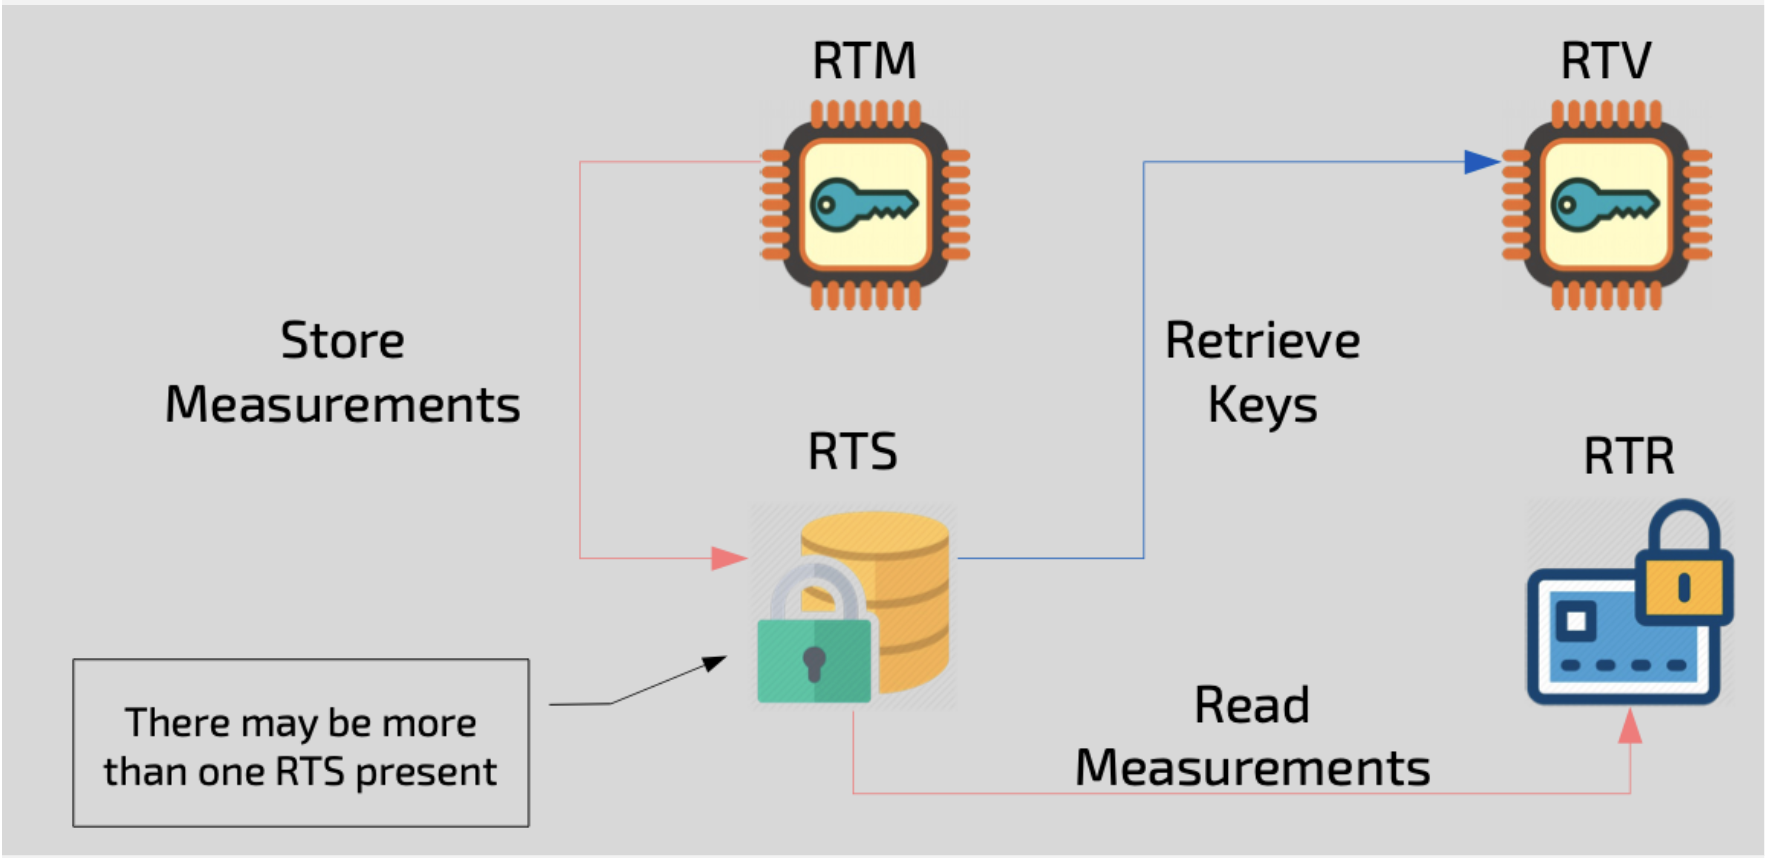
\includegraphics[width=0.8\textwidth]{./chapters/figures/TPM.png}
	\caption{TPM Architecture and Roots of Trust}
	\label{fig:TPM_architecture}
\end{figure}


\subsection{Certification and Attestation}
Certification and attestation are essential for establishing and 
verifying trust in TPM-enabled platforms. 

\textbf{Certification} uses cryptographic certificates to validate 
TPM components, starting with a key shipped with the TPM. 
This certified key forms the basis for a chain of trust, 
enabling secure storage and use of signing keys to prove system 
integrity.

\textbf{Attestation} allows the TPM to prove its state and 
authenticity to external entities, using unique identifiers 
(e.g., from Physical Unclonable Functions) and cryptographic 
evidence. Attestation covers compliance, the presence of trusted 
roots, and protection of key pairs.

Modern hierarchical attestation extends beyond one-time certification, 
enabling ongoing, layered verification of the platform’s 
trustworthiness, including the TPM, boot process, and system 
configuration.


\section{Tools for Implementation and Testing}
To implement and test the TPM from the hardware side, we used QEMU.

QEMU is an open-source machine emulator and virtualizer that 
allows you to test and run harware platforms and operating systems
in a virtualized environment.
It supports a wide range of architectures and can emulate various
hardware components, including CPUs, memory, and peripherals.
It is widely used for development, testing, and debugging purposes,
providing a flexible and efficient way to simulate hardware systems.
It is particularly useful for testing firmware and software in a 
controlled environment before deploying it on actual hardware.

In this case it was used to emulate the hardware platform, adding the 
TPM component to the emulated system. 